\documentclass[a4paper,twoside]{article}
% My LaTeX preamble file - by Nathaniel Dene Hoffman
% Credit for much of this goes to Olivier Pieters (https://olivierpieters.be/tags/latex)
% and Gilles Castel (https://castel.dev)
% There are still some things to be done:
% 1. Update math commands using mathtools package (remove ddfrac command and just override)
% 2. Maybe abbreviate \imath somehow?
% 3. Possibly format for margin notes and set new margin sizes
% First, some encoding packages and useful formatting
%--------------------------------------------------------------------------------------------
\usepackage{import}
\usepackage{pdfpages}
\usepackage{transparent}
\usepackage[l2tabu,orthodox]{nag}   % force newer (and safer) LaTeX commands
\usepackage[utf8]{inputenc}         % set character set to support some UTF-8
                                    %   (unicode). Do NOT use this with
                                    %   XeTeX/LuaTeX!
\usepackage[T1]{fontenc}
\usepackage[english]{babel}         % multi-language support
\usepackage{sectsty}                % allow redefinition of section command formatting
\usepackage{tabularx}               % more table options
\usepackage{booktabs}
\usepackage{titling}                % allow redefinition of title formatting
\usepackage{imakeidx}               % create and index of words
\usepackage{xcolor}                 % more colour options
\usepackage{enumitem}               % more list formatting options
\usepackage{tocloft}                % redefine table of contents, new list like objects
\usepackage{subfiles}               % allow for multifile documents

% Next, let's deal with the whitespaces and margins
%--------------------------------------------------------------------------------------------
\usepackage[centering,margin=1in]{geometry}
\setlength{\parindent}{0cm}
\setlength{\parskip}{2ex plus 0.5ex minus 0.2ex} % whitespace between paragraphs

% Redefine \maketitle command with nicer formatting
%--------------------------------------------------------------------------------------------
\pretitle{
  \begin{flushright}         % align text to right
    \fontsize{40}{60}        % set font size and whitespace
    \usefont{OT1}{phv}{b}{n} % change the font to bold (b), normally shaped (n)
                             %   Helvetica (phv)
    \selectfont              % force LaTeX to search for metric in its mapping
                             %   corresponding to the above font size definition
}
\posttitle{
  \par                       % end paragraph
  \end{flushright}           % end right align
  \vskip 0.5em               % add vertical spacing of 0.5em
}
\preauthor{
  \begin{flushright}
    \large                   % font size
    \lineskip 0.5em          % inter line spacing
    \usefont{OT1}{phv}{m}{n}
}
\postauthor{
  \par
  \end{flushright}
}
\predate{
  \begin{flushright}
  \large
  \lineskip 0.5em
  \usefont{OT1}{phv}{m}{n}
}
\postdate{
  \par
  \end{flushright}
}

% Mathematics Packages
\usepackage[Gray,squaren,thinqspace,cdot]{SIunits}      % elegant units
\usepackage{amsmath}                                    % extensive math options
\usepackage{amsfonts}                                   % special math fonts
\usepackage{mathtools}                                  % useful formatting commands
\usepackage{amsthm}                                     % useful commands for building theorem environments
\usepackage{amssymb}                                    % lots of special math symbols
\usepackage{mathrsfs}                                   % fancy scripts letters
\usepackage{cancel}                                     % cancel lines in math
\usepackage{esint}                                      % fancy integral symbols
\usepackage{relsize}                                    % make math things bigger or smaller
%\usepackage{bm}                                         % bold math!
\usepackage{slashed}

\newcommand\ddfrac[2]{\frac{\displaystyle #1}{\displaystyle #2}}    % elegant fraction formatting
\allowdisplaybreaks[1]                                              % allow align environments to break on pages

% Ensure numbering is section-specific
%--------------------------------------------------------------------------------------------
\numberwithin{equation}{section}
\numberwithin{figure}{section}
\numberwithin{table}{section}

% Citations, references, and annotations
%--------------------------------------------------------------------------------------------
\usepackage[small,bf,hang]{caption}        % captions
\usepackage{subcaption}                    % adds subfigure & subcaption
\usepackage{sidecap}                       % adds side captions
\usepackage{hyperref}                      % add hyperlinks to references
\usepackage[noabbrev,nameinlink]{cleveref} % better references than default \ref
\usepackage{autonum}                       % only number referenced equations
\usepackage{url}                           % urls
\usepackage{cite}                          % well formed numeric citations
% format hyperlinks
\colorlet{linkcolour}{black}
\colorlet{urlcolour}{blue}
\hypersetup{colorlinks=true,
            linkcolor=linkcolour,
            citecolor=linkcolour,
            urlcolor=urlcolour}

% Plotting and Figures
%--------------------------------------------------------------------------------------------
\usepackage{tikz}          % advanced vector graphics
\usepackage{pgfplots}      % data plotting
\usepackage{pgfplotstable} % table plotting
\usepackage{placeins}      % display floats in correct sections
\usepackage{graphicx}      % include external graphics
\usepackage{longtable}     % process long tables

% use most recent version of pgfplots
\pgfplotsset{compat=newest}

% Misc.
%--------------------------------------------------------------------------------------------
\usepackage{todonotes}  % add to do notes
\usepackage{epstopdf}   % process eps-images
\usepackage{float}      % floats
\usepackage{stmaryrd}   % some more nice symbols
\usepackage{emptypage}  % suppress page numbers on empty pages
\usepackage{multicol}   % use this for creating pages with multiple columns
\usepackage{etoolbox}   % adds tags for environment endings
\usepackage{tcolorbox}  % pretty colored boxes!


% Custom Commands
%--------------------------------------------------------------------------------------------
\newcommand\hr{\noindent\rule[0.5ex]{\linewidth}{0.5pt}}                % horizontal line
\newcommand\N{\ensuremath{\mathbb{N}}}                                  % blackboard set characters
\newcommand\R{\ensuremath{\mathbb{R}}}
\newcommand\Z{\ensuremath{\mathbb{Z}}}
\newcommand\Q{\ensuremath{\mathbb{Q}}}
%\newcommand\C{\ensuremath{\mathbb{C}}}
\renewcommand{\arraystretch}{1.2}                                       % More space between table rows (could be 1.3)
\newcommand{\Cov}{\mathrm{Cov}}
\newcommand\D{\mathrm{D}}
\newcommand*{\dbar}{\ensuremath{\text{\dj}}}

\newcommand{\incfig}[2][1]{%
    \def\svgwidth{#1\columnwidth}
    \import{./figures/}{#2.pdf_tex}
}

% Custom Environments
%--------------------------------------------------------------------------------------------
\newcommand{\lecture}[3]{\hr\\{\centering{\large\textsc{Lecture #1: #3}}\\#2\\}\hr\markboth{Lecture #1: #3}{\rightmark}}   % command to title lectures
\usepackage{mdframed}
\theoremstyle{plain}
\newmdtheoremenv[nobreak]{theorem}{Theorem}[section]
\newtheorem{corollary}{Corollary}[theorem]
\newtheorem{lemma}[theorem]{Lemma}
\theoremstyle{definition}
\newtheorem*{ex}{Example}
\newmdtheoremenv[nobreak]{definition}{Definition}[section]
\theoremstyle{remark}
\newtheorem*{remark}{Remark}
\newtheorem*{claim}{Claim}
\AtEndEnvironment{ex}{\null\hfill$\diamond$}%
% Note: A proof environment is already provided in the amsthm package
\tcbuselibrary{breakable}
\newenvironment{note}[1]{\begin{tcolorbox}[
    arc=0mm,
    colback=white,
    colframe=white!60!black,
    title=#1,
    fonttitle=\sffamily,
    breakable
]}{\end{tcolorbox}}
\newenvironment{problem}{\begin{tcolorbox}[
    arc=0mm,
    breakable,
    colback=white,
    colframe=black
]}{\end{tcolorbox}}

% Header and Footer
%--------------------------------------------------------------------------------------------
% set header and footer
\usepackage{fancyhdr}                       % header and footer
\pagestyle{fancy}                           % use package
\fancyhf{}
\fancyhead[LE,RO]{\textsl{\rightmark}}      % E for even (left pages), O for odd (right pages)
\fancyfoot[LE,RO]{\thepage}
\fancyfoot[LO,RE]{\textsl{\leftmark}}
\setlength{\headheight}{15pt}


% Physics
%--------------------------------------------------------------------------------------------
\usepackage[arrowdel]{physics}      % all the usual useful physics commands
\usepackage{feyn}                   % for drawing Feynman diagrams
%\usepackage{bohr}                   % for drawing Bohr diagrams
%\usepackage{tikz-feynman}
\usepackage{elements}               % for quickly referencing information of various elements
\usepackage{tensor}                 % for writing tensors and chemical symbols

% Finishing touches
%--------------------------------------------------------------------------------------------
\author{Nathaniel D. Hoffman}

\title{33-755 Homework 3}
\date{\today}
\begin{document}
\maketitle
\section{Spin States on the Bloch Sphere}%
\label{sec:spin_states_on_the_bloch_sphere}

The unit vector $\mathbf{n}$ with polar angle $\theta$ and azimuthal angle $\phi$ has Cartesian coordinates $(\sin\theta\cos\phi,\sin\theta\sin\phi,\cos\theta)$. Let $S_x = \frac{\hbar}{2}\sigma_x$, $S_y = \frac{\hbar}{2}\sigma_y$, $S_z = \frac{\hbar}{2}\sigma_z$ be the $x$, $y$, and $z$ components of the spin operator $\mathbf{S}$.
\begin{itemize}
    \item[a)] Express the operator $S_n\equiv\mathbf{n}\cdot \mathbf{S}$ as a matrix in the $\{\pm z\} $ basis.

\begin{tcolorbox}
    \begin{equation}
        S_n = \frac{\hbar}{2}\left[(\sin\theta\cos\phi)\sigma_x + (\sin\theta\sin\phi)\sigma_y + (\cos\theta)\sigma_z  \right]
    \end{equation}
    Given that the Pauli matrices are
    \begin{align*}
        \sigma_x &= \begin{pmatrix} 0&1\\1&0 \end{pmatrix}\\
        \sigma_y &= \begin{pmatrix} 0&-\imath\\ \imath&0 \end{pmatrix}\\
        \sigma_z &= \begin{pmatrix} 1&0\\0&-1 \end{pmatrix} 
    .\end{align*}
    we find that the matrix representation of $S_n$ is
    \begin{equation}
        S_n = \frac{\hbar}{2}\begin{bmatrix} \cos\theta & \sin\theta\cos\phi -\imath\sin\theta\sin\phi \\ \sin\theta\cos\phi + \imath\sin\theta\sin\phi & -\cos\theta  \end{bmatrix}
    \end{equation}
    or
    \begin{equation}
        S_n = \frac{\hbar}{2}\begin{bmatrix} \cos\theta & e^{-\imath\phi}\sin\theta \\ e^{\imath\phi}\sin\theta & -\cos\theta \end{bmatrix}  
    \end{equation}
\end{tcolorbox}

    \item[b)] $S_n$ has two eigenvectors that we shall denote $\ket{n+}$ and $\ket{n-}$. Determine these eigenvectors and their corresponding eigenvalues.

\begin{tcolorbox}
    First, we can find the eigenvalues by computing the characteristic polynomial:
    \begin{equation}
        \left(\frac{\hbar}{2}\cos\theta-\lambda\right)\left(-\frac{\hbar}{2}\cos\theta-\lambda\right)-\left(\frac{\hbar}{2}\right)^2\sin^2\theta = 0
    \end{equation}
    or
    \begin{equation}
        \lambda^2-\left(\frac{\hbar}{2}\right)^2\left(\sin^2\theta + \cos^2\theta  \right) = 0 
    \end{equation}
    so
    \begin{equation}
        \lambda = \pm\frac{\hbar}{2}
    \end{equation}

    We can find the first eigenvector, corresponding to $\lambda = +\frac{\hbar}{2}$, as follows:

    \begin{equation}
        \frac{\hbar}{2} \begin{bmatrix}x\cos\theta+ye^{-\imath\phi}\sin\theta \\ -y\cos\theta + x e^{\imath\phi}\sin\theta \end{bmatrix} = \frac{\hbar}{2}\begin{bmatrix} x\\y \end{bmatrix}
    \end{equation}
    Using the first equation given in this system, we see that
    \begin{equation}
        x(\cos\theta - 1) = -ye^{-\imath\phi}\sin\theta
    \end{equation}
    or
    \begin{align*}
        x e^{\imath\phi} &= -y\frac{\sin\theta}{\cos\theta - 1}\\
        &= y \frac{\cos \frac{\theta}{2}}{\sin \frac{\theta}{2}}\\
        x e^{\imath\phi}\sin \frac{\theta}{2} &= y\cos \frac{\theta}{2}
    .\end{align*}
    so we can make our first eigenvector
    \begin{equation}
        \ket{n+} = \begin{pmatrix} \cos \frac{\theta}{2}\\ e^{\imath\phi}\sin \frac{\theta}{2} \end{pmatrix} 
    \end{equation}
    By doing the same procedure with the other eigenvalue, we find that for $\lambda = -\frac{\hbar}{2}$,
\begin{equation}
    \ket{n-} = \begin{pmatrix} -e^{\imath\phi}\sin \frac{\theta}{2}\\ \cos \frac{\theta}{2} \end{pmatrix} 
\end{equation}
We can also find this second result from the fact that the eigenvalues are non-degenerate, so the eigenvectors will be orthogonal.
\end{tcolorbox}

\end{itemize}

\section{Spin in Constant Magnetic Field}%
\label{sec:spin_in_cons}

The following problem is adapted from Cohen-Tannoudji, chapter 4. Consider a spin-$\frac{1}{2}$ particle in a constant magnetic field tilted slightly away from the $z$-axis in the $yz$-plane. The Hamiltonian
\begin{equation}
    H = \frac{1}{2}\left( \omega_y\sigma_y + \omega_z\sigma_z \right) 
\end{equation}
\begin{itemize}
    \item[a)] Express $H$ as a matrix in the standard basis $ \{\ket{z+},\ket{z-}\}$.
\begin{tcolorbox}
    \begin{align*}
        H &= \frac{1}{2}\left( \omega_y \begin{pmatrix} 0&-\imath \\ \imath & 0 \end{pmatrix} + \omega_z \begin{pmatrix} 1&0\\0&-1 \end{pmatrix} \right)\\
        &= \frac{1}{2} \begin{pmatrix} \omega_z & -\imath\omega_y \\ \imath\omega_y & -\omega_z \end{pmatrix} 
    .\end{align*}
\end{tcolorbox}
    \item[b)] Express the eigenvalues and eigenvectors of $H$ as explicit superpositions within the standard basis.
        \begin{tcolorbox}[breakable]
    First, we need to find the eigenvalues and eigenvectors. The characteristic equation for this system is:
    \begin{equation}
        \left(\frac{\omega_z}{2}-\lambda\right)\left(-\frac{\omega_z}{2}-\lambda\right) - \frac{\omega_y^2}{4} = 0
    \end{equation}
    or
    \begin{equation}
        \lambda^2 = \frac{\omega_y^2}{4} + \frac{\omega_z^2}{4} 
    \end{equation}
    so
    \begin{equation}
        \lambda = \pm\frac{1}{2}\sqrt{\omega_y^2 + \omega_z^2} 
    \end{equation}
    Now, we calculate the first (positive eigenvalue) eigenvector. I will, in advance, multiply both sides of the equation by $2$ so I don't have to keep writing a fraction that I will cancel anyway:
    \begin{align*}
        \begin{bmatrix} \omega_z x - \imath\omega_y y \\ \imath\omega_y x -\omega_z y \end{bmatrix} &= \begin{bmatrix} x\sqrt{\omega_y^2 + \omega_z^2} \\ y\sqrt{\omega_y^2+\omega_z^2} \end{bmatrix}\\
        \implies x\left( \omega_z - \sqrt{\omega_y^2 + \omega_z^2} \right) &= \imath\omega_y y
    .\end{align*}
    so our first eigenvector could be
    \begin{equation}
        \begin{pmatrix} \imath\omega_y \\ \omega_z-\sqrt{\omega_y^2+\omega_z^2}  \end{pmatrix} 
    \end{equation}
    In a form showing the superposition of states in the standard basis, this would be:
    \begin{equation}
        \ket{\lambda+} = \imath\omega_y\ket{z+} + \left(\omega_z-\sqrt{\omega_y^2+\omega_z^2}\right)\ket{z-}
    \end{equation}
    The other eigenvector is
    \begin{equation}
        \ket{\lambda-} =  \imath\omega_y \ket{z+} + \left( \omega_z + \sqrt{\omega_0^2 + \omega_z^2}  \right)\ket{z-}
    \end{equation}
\end{tcolorbox}
    \item[c)] On a single set of axes, sketch the eigenvalues of $H$ as functions of $\omega_z$ (consider both positive and negative values). Include both the case $\omega_y = 0$ and the case $\omega_y > 0$.
\begin{tcolorbox}[breakable]
    Our equations for the eigenvalues were
    \begin{equation}
        \lambda = \pm\frac{1}{2}\sqrt{\omega_y^2+\omega_z^2}.
    \end{equation}
\end{tcolorbox}
\begin{figure}[h]
    \centering
    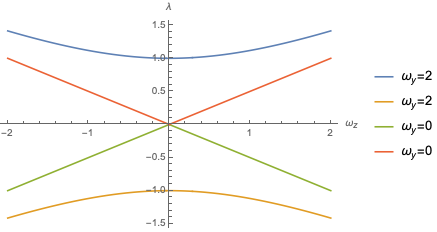
\includegraphics[width=0.8\textwidth]{plot_hw3_2c.png}
    \caption{Plot of $\lambda$ vs $\omega_z$ with select values of $\omega_y\ge 0$.}
    \label{fig:plot2c}
\end{figure}

    \item[d)] Expand the eigenvalues as power series in $\omega_z$, keeping only the lowest nonzero power of $\omega_z$. Treat both the case $\omega_y = 0$ and the case $\omega_y > 0$.
\begin{tcolorbox}[breakable]
    The first two derivatives of $\frac{1}{2}\sqrt{\omega_y^2+\omega_z^2}$ with respect to $\omega_z$ are:
    \begin{align*}
        f'(\omega_z) &= \frac{\omega_z}{2\sqrt{\omega_y^2+\omega_z^2} }\\
        f''(\omega_z) &= \frac{1}{2\sqrt{\omega_y^2+\omega_z^2} }- \frac{\omega_z^2}{2\left(\omega_y^2+\omega_z^2 \right)^{\frac{3}{2}} }
    .\end{align*}
    Evaluating at $\omega_z = 0$, we most of the terms in both go to zero, and we are only left with
    \begin{equation}
        f''(0)=\frac{1}{2\sqrt{\omega_y^2} }
    \end{equation}
    The power series expansion is therefore
    \begin{align*}
        \lambda &= (\pm)\left( f(0) + f'(0)x + \frac{1}{2}f''(0)x^2 \right)\\
                &= (\pm)\left( \frac{\omega_y}{2} + \frac{\omega_z^2}{4\omega_y} + \mathcal{O}[\omega_z]^4  \right) 
    .\end{align*}
    (there are no odd powers of $\omega_z$). When $\omega_y = 0$, we see that
\begin{equation}
    \lambda = (\pm) \frac{\omega_z}{2}.
\end{equation}
\end{tcolorbox}
    \item[e)] Letting the initial state $\ket{\psi_0} = \ket{z+}$, determine the time-evolved state $\ket{\psi(t)}$. Hint: it may be convenient to express $\ket{\psi(t)}$ in the basis of eigenstates of the Hamiltonian.
        \begin{tcolorbox}[breakable]
            Since the Hamiltonian is time independent, we can define a unitary time evolution operator
            \begin{equation}
                U = e^{\frac{\imath Ht}{\hbar}} 
            \end{equation}
            From here, we will take the hint to write our state in terms of the eigenstates of the Hamiltonian:
\begin{equation}
    \ket{\lambda+} = \imath\omega_y\ket{z+} + \left(\omega_z-\sqrt{\omega_y^2+\omega_z^2}\right)\ket{z-}
\end{equation}
\begin{equation}
    \ket{\lambda-} = \imath\omega_y \ket{z+} + \left( \omega_z + \sqrt{\omega_0^2 + \omega_z^2}  \right) \ket{z-}
\end{equation}
We can rewrite the eigenstates as
\begin{align*}
    \ket{\lambda+}&=\ket{z+}+ \frac{\omega_z-\sqrt{\omega_y^2+\omega_z^2}}{\imath\omega_y}\ket{z-}\\
    \ket{\lambda-}&= \frac{\imath\omega_y}{\omega_z+\sqrt{\omega_y^2+\omega_z^2} } + \ket{z-}\\
        \ket{z+}&=\ket{\lambda+}- \frac{\omega_z-\sqrt{\omega_y^2+\omega_z^2}}{\imath\omega_y}\ket{z-}\\
        \ket{z-}&=\ket{\lambda-} - \frac{\imath\omega_y}{\omega_z+\sqrt{\omega_y^2+\omega_z^2}}\ket{z+}\\
        \ket{z+}&=\ket{\lambda+}- \frac{\omega_z-\sqrt{\omega_y^2+\omega_z^2}}{\imath{\omega_y}}\left[\ket{\lambda-}+ \frac{\imath\omega_y}{\omega_z + \sqrt{\omega_y^2+\omega_z^2}}\ket{z+}\right]\\
        &=\ket{\lambda+}- \frac{\omega_z-\sqrt{\omega_y^2+\omega_z^2}}{\imath\omega_y}\ket{\lambda-} + \frac{\omega_z-\sqrt{\omega_y^2+\omega_z^2}}{\omega_z+\sqrt{\omega_y^2+\omega_z^2}}\ket{z+}\\
        &\cancelto{\left( \frac{2\sqrt{\omega_y^2+\omega_z^2}}{\omega_z+\sqrt{\omega_y^2+\omega_z^2}}\right)}{\left(1- \frac{\omega_z-\sqrt{\omega_y^2+\omega_z^2}}{\omega_z + \sqrt{\omega_y^2+\omega_z^2}}\right)}\ket{z+} = \ket{\lambda+} - \frac{\omega_z-\sqrt{\omega_y^2+\omega_z^2}}{\imath\omega_y}\ket{\lambda-}\\
        \ket{z+}&= \frac{\omega_z+\sqrt{\omega_y^2+\omega_z^2}}{2\sqrt{\omega_y^2+\omega_z^2}}\ket{\lambda+} + \frac{\omega_y}{2\imath\sqrt{\omega_y^2+\omega_z^2} }\ket{\lambda-} 
.\end{align*}

What was the purpose of this? The operator $U$, when acting on an eigenstate of $H$, will return the original state multiplied by $e^{\frac{\imath\lambda t}{\hbar}}$, where $\lambda$ is the eigenvalue of that state. We can now act this operator on our state:
\begin{align*}
    &U\ket{\psi_0} = U\ket{z+} = e^{\frac{\imath\lambda^+ t}{\hbar}} \frac{\omega_z+\sqrt{\omega_y^2+\omega_z^2}}{2\sqrt{\omega_y^2+\omega_z^2}}\ket{\lambda+}\\ &+ e^{\frac{\imath\lambda^- t}{\hbar}}\frac{\omega_y}{2\imath\sqrt{\omega_y^2+\omega_z^2} }\ket{\lambda-}\\
    &=e^\mu \frac{\omega_z + \sqrt{\omega_y^2+\omega_z^2}}{2\sqrt{\omega_y^2+\omega_z^2}}\left( \ket{z+} + \frac{\omega_z - \sqrt{\omega_y^2+\omega_z^2}}{\imath \omega_y}\ket{z-} \right)\\ &+ e^\nu \frac{\omega_y}{2\imath \sqrt{\omega_y^2+\omega_z^2}}\left( \frac{\imath\omega_y}{\omega_z + \sqrt{\omega_y^2+\omega_z^2}}\ket{z+} + \ket{z-} \right)\\  
    &= \left( e^\mu \frac{\omega_z+\sqrt{\omega_y^2+\omega_z^2}}{2\sqrt{\omega_y^2+\omega_z^2}} + e^\nu \frac{\omega_y}{2\imath\sqrt{\omega_y^2+\omega_z^2}} \frac{\imath\omega_y}{\omega_z + \sqrt{\omega_y^2+\omega_z^2}}\ket{z+}  \right)\\ &+ \left( e^\mu \frac{\omega_z+\sqrt{\omega_y^2+\omega_z^2}}{2\sqrt{\omega_y^2+\omega_z^2}} \frac{\omega_z-\sqrt{\omega_y^2+\omega_z^2}}{\imath\omega_y}+e^\nu \frac{\omega_y}{2\imath\sqrt{\omega_y^2+\omega_z^2}}\ket{z-}\right)\\
    &=\left( e^\mu \frac{\omega_z+\sqrt{\omega_y^2+\omega_z^2}}{2\sqrt{\omega_y^2+\omega_z^2}} + e^\nu \frac{\omega_y^2}{2\sqrt{\omega_y^2+\omega_z^2}(\omega_z+\sqrt{\omega_y^2+\omega_z^2})} \right)\ket{z+}\\ &+ \left( e^\nu - e^\mu \right)\left( \frac{\omega_y}{2\imath\sqrt{\omega_y^2+\omega_z^2}} \right)\ket{z-} = \ket{\psi(t)}
.\end{align*}
where $e^\mu = e^{\frac{\imath \sqrt{\omega_y^2+\omega_z^2}t}{2\hbar}}$ and $e^\nu = e^{-\frac{\imath \sqrt{\omega_y^2+\omega_z^2}t}{2\hbar}}$
\end{tcolorbox}
    \item[f)] Calculate the probability $P_{-+}(t)$ of spin down $\ket{z-}$ at time $t$ given the initial spin up state $\ket{z+}$ at time $0$. Sketch this probability over one full period of Rabi oscillation. Be sure to label your axes with characteristic times and probabilities.
\begin{tcolorbox}[breakable]
    \begin{equation}
        P_{-+}(t) = \ip{\psi(t)}{z-}\ip{z-}{\psi(t)}
    \end{equation} 
    Only the part associated with $\ket{z-}$ survives the dyad, so we have
    \begin{equation}
        P = (e^\nu - e^\mu)\left( \frac{\omega_y}{2\imath\sqrt{\omega_y^2+\omega_z^2} } \right) (e^{-\nu} - e^{-\mu})\left( \frac{-\omega_y}{2\imath\sqrt{\omega_y^2+\omega_z^2} } \right)
    \end{equation}
    (maintaining the same shorthand for $\mu$ and $\nu$ for now). Finally, multiplying these terms out gives us
    \begin{equation}
        P_{-+}(t) = \left( \frac{\omega_y^2}{4(\omega_y^2+\omega_z^2)} \right) \left( 2-e^{\imath\sqrt{\omega_y^2+\omega_z^2}\frac{t}{\hbar}} - e^{-\imath\sqrt{\omega_y^2+\omega_z^2}\frac{t}{\hbar}} \right) 
    \end{equation}
    We can simplify the exponential further:
    \begin{equation}
    P_{-+}(t) = \left( \frac{\omega_y^2}{2(\omega_y^2+\omega_z^2)} \right) \left( 1-\cos(\sqrt{\omega_y^2+\omega_z^2}\frac{t}{\hbar})\right)
    \end{equation}

    As shown in the plot, the characteristic time for the maximum probability occurs when $1-\cos$ is maximum, which happens when $\cos = -1$. This corresponds to the argument being $\pi$, so $t_\text{max} = \frac{\pi}{\sqrt{\omega_y^2 + \omega_z^2} }$. The maximum height is determined by $\frac{\omega_y^2}{2\omega_y^2+\omega_z^2}$, and when $\omega_y = 0$, we see that there is no probability to switch to the $\ket{z+}$ state because the $\ket{z-}$ state is aligned with the only magnetic field. Similarly, if $\omega_z = 0$, the equation reduces further, and the maximum probability of finding a particle in either state is $\frac{1}{2}$, while the characteristic time to get this probability is nopi$\frac{\pi}{\omega_y}$. In this explanation I have assumed natural units: $\hbar = 1$.
\end{tcolorbox}
\begin{figure}[h]
    \centering
    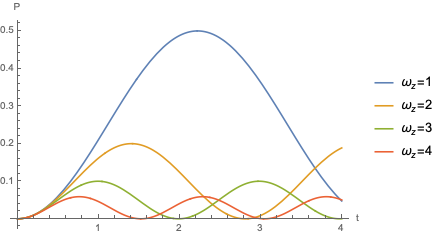
\includegraphics[width=0.8\textwidth]{plot_hw3_2f.png}
    \caption{Plot of Probability vs Time for select values of $\omega_z$ ($\omega_y = 1$)}
    \label{fig:plot2f}
\end{figure}
\end{itemize}


\section{Quantum States}%
\label{sec:quantum_states}

\begin{itemize}
    \item[a)] Let $Q$ be a spin-$ \frac{1}{2}$ particle with magnetic moment $\bm{\mu} = \gamma \bm{S} = \frac{\hbar}{2}\gamma\bm{\sigma}$. A static magnetic field of strength $B$ acts in the direction $\mathbf{\hat{n}}$ for a period of time $\tau$. Determine the direction $\mathbf{\hat{n}}$ and the time interval $\tau_\mathcal{H}$ such that the unitary time evolution operator expressed in the $\{\ket{z^\pm}\} $ basis (up to an irrelevant complex phase factor) is
\begin{equation}
    \mathcal{H} = \frac{1}{\sqrt{2} }\begin{pmatrix} 1&1\\1&-1 \end{pmatrix} 
\end{equation}

How does this transformation, known as the Hadamard transformation, act on the states $\{\ket{x^\pm}\} $, $\{\ket{y^\pm}\} $, and $\{\ket{z^\pm}\} $ of $Q$? What happens if you evolve for time $2\tau_\mathcal{H}$?

\begin{tcolorbox}[breakable]
    We start by remarking that our Hamiltonian is $H=-\bm{\mu}\cdot \bm{\hat{n}}B$ and $\mathcal{H} = e^{-\imath \frac{t}{\hbar}H}$ so we can start by taking the natural logarithm of the given unitary time evolution operator and relate it to the known Hamiltonian in terms of coordinates on the Bloch Sphere (from Problem 1):
    \begin{equation}
        \ln(\mathcal{H}) = -\imath \frac{t}{\hbar}\gamma B \frac{\hbar}{2}\begin{bmatrix} \cos\theta & e^{\imath\phi}\sin\theta \\ e^{-\imath\phi}\sin\theta & -\cos\theta  \end{bmatrix}
    \end{equation}
    
    Doing the calculation on the left-hand side yields:
    \begin{equation}
        \frac{\imath\pi}{2}\begin{bmatrix} 1-\frac{\sqrt{2}}{2} & -\frac{\sqrt{2}}{2} \\ -\frac{\sqrt{2}}{2} & 1 + \frac{\sqrt{2}}{2}      \end{bmatrix} = -\imath \frac{t}{\hbar}\gamma B \frac{\hbar}{2}\begin{bmatrix} \cos\theta & e^{\imath\phi}\sin\theta \\ e^{-\imath\phi}\sin\theta & -\cos\theta  \end{bmatrix} 
    \end{equation}
    Because our solution is not unique to a phase, we will consider one which adds $\frac{\pi}{2}$ to our unitary operator, allowing us to get rid of the $1$'s on the left-hand side:
    \begin{equation}
        \pi\begin{bmatrix} \frac{\sqrt{2}}{2} & \frac{\sqrt{2}}{2} \\ \frac{\sqrt{2}}{2} & -\frac{\sqrt{2}}{2} \end{bmatrix} = t\gamma B \begin{bmatrix} \cos\theta & e^{\imath\phi}\sin\theta \\ e^{-\imath\phi}\sin\theta & -\cos\theta  \end{bmatrix}
    \end{equation}
It's clear to see now that we require $\phi = 0$, which allows us to solve for $\theta = \frac{\pi}{4}$. Additionally, we find $\tau_\mathcal{H} =\frac{\pi}{\gamma B}$

Evolving for time $\tau_\mathcal{H}$ is just acting the operator $\mathcal{H}$ on the state, and evolving it for twice that time is equivalent to acting the operator on the state twice:
\begin{equation}
    \mathcal{H}\ket{x^\pm} = \frac{1}{2}\begin{pmatrix} 1&1\\1&-1 \end{pmatrix} \begin{pmatrix} 1\\ \pm 1 \end{pmatrix} = \ket{z^\pm}
\end{equation}

As we might imagine,
\begin{equation}
    \mathcal{H}\ket{z^\pm} = \ket{x^\pm}
\end{equation}

Acting it on the $\ket{y^\pm}$ states, we find:
\begin{equation}
    \mathcal{H}\ket{y^\pm} = \frac{1}{2}\begin{pmatrix} 1\pm\imath \\ 1\mp\imath \end{pmatrix} 
\end{equation}

Acting the operator on the $\ket{x^\pm}$ and $\ket{z^\pm}$ identifies them back to themselves ($\mathcal{H}(2\tau_\mathcal{H}) = \mathcal{H}(\tau_\mathcal{H})\circ\mathcal{H}(\tau_\mathcal{H})$). For the $\ket{y^\pm}$ states, we also find that
\begin{equation}
    \mathcal{H}\mathcal{H}\ket{y^\pm} = \mathcal{H} \frac{1}{2}\begin{pmatrix} 1\pm\imath \\ 1\mp\imath \end{pmatrix} = \ket{y^\pm}
\end{equation}
\end{tcolorbox}

    \item[b)] Let $Q_1$ and $Q_2$ be identical spin-$\frac{1}{2}$ particles. They interact with a magnetic field in the $\hat{z}$ direction, and with each other, for a duration $\tau$ under the Hamiltonian
\begin{equation}
    H_\mathcal{Z} = \frac{1}{2}(\hbar\omega_0)\left( -I+\sigma_z^{(1)} + \sigma_z^{(2)} - \sigma_z^{(1)} \otimes \sigma_z^{(2)} \right).
\end{equation}
Here superscripts indicate the individual spins, and tensor products with identity operators are implicit where needed. Determine the time interval $\tau_\mathcal{Z}$ for which the unitary time evolution operator (expressed in the basis $\{z^\pm z^\pm\} $) is
\begin{equation}
    \mathcal{Z} = \begin{pmatrix} 1&0&0&0\\0&1&0&0\\0&0&1&0\\0&0&0&-1\end{pmatrix}.
\end{equation}
This transformation is known as a controlled $Z$ gate.
\begin{tcolorbox}[breakable]
    We can start by writing the matrix form of the Hamiltonian:
    \begin{align*}
        H_\mathcal{Z} &= \frac{1}{2}(\hbar\omega_0)\left(\begin{pmatrix} -1&0&0&0\\0&-1&0&0\\0&0&-1&0\\0&0&0&-1 \end{pmatrix}\right.\\
    &+ \begin{pmatrix} 1&0&0&0\\0&1&0&0\\0&0&-1&0\\0&0&0&-1 \end{pmatrix}\\
&+ \begin{pmatrix} 1&0&0&0\\0&-1&0&0\\0&0&1&0\\0&0&0&-1 \end{pmatrix}\\
&+\left. \begin{pmatrix} -1&0&0&0\\0&1&0&0\\0&0&1&0\\0&0&0&-1 \end{pmatrix} \right)\\
&=(\hbar\omega_0)\begin{pmatrix}0&0&0&0\\0&0&0&0\\0&0&0&0\\0&0&0&-2 \end{pmatrix} 
    .\end{align*}

    We can now relate this to the logarithm of the given unitary time evolution operator:
    \begin{equation}
        \ln(\mathcal{Z}) = \begin{pmatrix}0&0&0&0\\0&0&0&0\\0&0&0&0\\0&0&0&\imath\pi\end{pmatrix} = -\imath \frac{\tau_\mathcal{Z}}{\hbar}H_\mathcal{Z}
    \end{equation}
    
    We can relate these through their last element:
    \begin{equation}
        \imath\pi = 2\imath \frac{\tau_\mathcal{Z}}{\hbar} \hbar\omega_0 \implies\tau_\mathcal{Z} = \frac{\pi}{2\omega_0}
    \end{equation}
\end{tcolorbox}

    \item[c)] In the tensor product space of $Q_1$ and $ Q_2$, apply the sequence of operations: $\mathcal{H}$ on $Q_2$, followed by $\mathcal{Z}$ on $Q_1\otimes Q_2$, followed by $\mathcal{H}^\dagger$ on $Q_2$. Express the combined action as a matrix taking the basis states in the following order $\{\ket{z^+z^+},\ket{z^+z^-},\ket{z^-z^+},\ket{z^-z^-}\} $. Why do we name this combination “controlled not”?

This question was inspired by reading a recent Physics Today article “Quantum computing with semiconductor spins” (see https://doi.org/10.1063/PT.3.4270) and was designed with help from Vikesh Siddhu.
\begin{tcolorbox}[breakable]
    We can create a combined set of matrices for $\mathcal{H}$ in the two-particle basis:
    \begin{equation}
        I\otimes\mathcal{H}^\dagger =\frac{1}{\sqrt{2}} \begin{pmatrix} 1&1&0&0\\1&-1&0&0\\0&0&1&1\\0&0&1&-1 \end{pmatrix} 
    \end{equation}
    Taking the product of all these matrices, we find a combined action matrix:
    \begin{equation}
        \mathcal{N} = \mathcal{H}^\dagger_{(2)}\mathcal{Z}\mathcal{H}_{(2)} =\frac{1}{2} \begin{pmatrix} 1&0&0&0\\0&1&0&0\\0&0&0&1\\0&0&1&0 \end{pmatrix} 
    \end{equation}
    Acting this on each basis state, we see that $\ket{++}\xrightarrow{\mathcal{N}}\ket{++}$, $\ket{+-}\xrightarrow{\mathcal{N}}\ket{+-}$, $\ket{-+}\xrightarrow{\mathcal{N}}\ket{--}$, and $\ket{--}\xrightarrow{\mathcal{N}}\ket{-+}$. This operation is a not function on the second state controlled by the first state. If the first particle is spin-up, the operation acts like the identity on the second particle. However, if the first particle is spin-down, the operation switches the spin of the second particle.
\end{tcolorbox}

\end{itemize}

\end{document}
